\documentclass[../main.tex]{subfiles}

\begin{document}

\subsection{Overview}
    
En este sección se detalla el proceso de compilación, entrenamiento y posterior conversión a CoreML para su uso en un dispositivo iOS.

Se realiza bajo los siguientes componentes y herramientas:
\begin{itemize}
    \item sistema operativo Ubuntu 20.04.1 LTS
    \item Entorno virtual Anacoda \cite{anaconda} para las instalación de herramientas a utilizar.
    \item Jupyter \cite{jupyter} como IDE para la programación del modelo de Deep Learning.
\end{itemize}

En el directorio con los datos del modelo, se incluye el fichero .yaml que incluye los paquetes necesarios para la configuración del entorno virtual a utilizar. De esta forma puede ser creado fácilmente el entorno virtual con la configuración deseada con la ejecución de este comando:


\begin{lstlisting}[style=swift]
conda env create --file=kerasenv.yaml
\end{lstlisting}

El entorno utiliza los siguientes paquetes:
\begin{lstlisting}[style=stylepython]
name: kerasenvTFGExtractedFeatures
channels:
  - defaults
dependencies:
  - python=3.6.8
  - pip
  - scikit-learn
  - scikit-image
  - matplotlib
  - seaborn
  - ipython
  - jupyter
  - scipy
  - numpy
  - pandas
  - pillow
  - pydot
  - keras=2.2.4
  - tensorflow=1.14
  - nomkl
  - pip:
    - coremltools==3.0
\end{lstlisting}


Es especialmente importante las versiones utilizadas de TensorFlow \cite{tensorflow} y Keras \cite{keras}, puesto que la sintaxis del lenguaje cambia bastante entre versiones y no funcionará correctamente sin modificaciones en versiones posteriores.

\subsection{Preparación de los datos de entrenamiento}
La ejecución del notebook de Jupyter se encuentra en los apéndices del documento \ref{notebook}, aquí se va a comentar los aspectos fundamentales de la construcción del modelo.

En el siguiente  fragmento de código definimos las etiquetas que se van a interpretar, así como el directorio 'Dataset\_short\_v3', que contiene una carpeta train con las características obtenidas por la aplicación de entrenamiento. 

Tras el procesado de datos, cada entrada de la variable X, es un vector de 42 valores representando las coordenadas de una letra. En el mismo índice de la variable Y, se encuentra la letra que representa esta entrada.

Para representar la letra, se utiliza un vector que utiliza one hot encoding. Esto significa que si estamos interpretando 24 letras, cada letra se representa como un vector de 24 posiciones, donde el índice de la letra que representa tiene el valor 1, y el resto el valor 0. Se muestra un ejemplo de la representación de la letra A y la letra X en la figura \ref{figure14}

\begin{lstlisting}[style=stylepython]
labels = ["A", "B", "C", "D", "E", "F", "G", "H", "I", "K",
        "L", "M", "N", "O", "P", "Q", "R", "S", "T", "U",
        "V", "W", "X", "Y"]
num_classes = len(labels)

data_dir = "Dataset_short_v3"
train_dir = os.path.join(data_dir, "train")
batch_size = 32

# X: features list, Y: class list to predict
X = []
Y = []

# read each folder of train
for label in labels:
    name = os.path.join(train_dir, label, label + ".csv")
    df = pd.read_csv(name)
    X.extend(df.values)
    newSize = len(df)
    print("Letter %s: num_data: %d" %( label, newSize))
    for i in range(0,newSize):
        Y.append(label)
    
# convert to np array to have shape
X = np.array(X)
Y = np.array(Y)

#one hot encoding
lb = preprocessing.LabelBinarizer()
lb.fit(labels)
Y = lb.transform(Y)
\end{lstlisting}

\begin{figure}[h]
\centering 
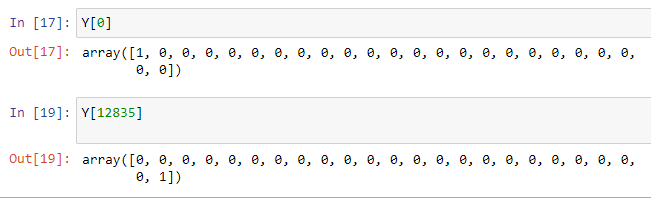
\includegraphics[width=0.9\textwidth]{images/modelo/oneehotencoding.PNG}
\caption{One hot encoding de las letras A,X.}
\label{figure14}
\end{figure}

Se dividen los datos de entrada en tres sets: datos de entrenamiento, validación y test. 

A cada letra se le establece un peso que determina la importancia de cada entrada  de una letra en el entrenamiento del modelo. El dataset utilizado no está balanceado en el número de datos de entrada por cada letra. Esto se debe a que se ha realizado un proceso de selección en los datasets utilizados, y algunas letras tenían muy pocas imágenes válidas para el entrenamiento. A las clases con menos datos de entrada, se le da más importancia a cada entrada en el entrenamiento del modelo.

\begin{lstlisting}[style=stylepython]
#split into training,val data. test_data
from sklearn.model_selection import train_test_split
X_train, X_test, Y_train, Y_test = train_test_split(X, Y, test_size=0.05)
X_train, X_val, Y_train, Y_val = train_test_split(X_train, Y_train, test_size=0.05)

#handle unbalance data 
Y_train_classes = lb.inverse_transform(Y_train)
from sklearn.utils import class_weight 
class_weights = class_weight.compute_class_weight('balanced',
                                                 np.unique(Y_train_classes),
                                                 Y_train_classes)
class_weight_dic = dict(enumerate(class_weights))
\end{lstlisting}

\newpage

\subsection{Compilación del modelo}
La configuración del modelo será una red neuronal que contiene las siguientes capas:
\begin{enumerate}
    \item Dense: Cada entrada es un vector de 42 valores y utiliza la función de activación 'relu'
    \item Dense: Esta capa recibe como entrada la salida de la capa anterior, y está formada por 24 clases, una que representa a cada letra.
    \item Activation: esta capa utiliza la función de activación 'softmax' y convierte cada entrada en una distribución de probabilidad en el que establece para cada tipo de letra, cual es la probabilidad de que la entrada inicial al modelo represente esa letra.
\end{enumerate}

Los hiper parámetros han sido seleccionados tras realizar varias pruebas y son los siguientes:
\begin{itemize}
    \item Función de optimización: Stochastic gradient descent.
    \item Learning rate: 0.01.
    \item Función de pérdida: Stochastic gradient descent
\end{itemize}
\begin{lstlisting}[style=stylepython]
model = Sequential()
model.add(Dense(32, activation='relu', input_shape=(42,)))
model.add(Dense(num_classes))
model.add(Activation("softmax"))

model.compile(optimizer=optimizers.SGD(lr=0.01), loss="Stochastic gradient descent",
                  metrics=["accuracy"])
\end{lstlisting}

Esto produce un modelo con un total de 2,168 parámetros que pueden ser entrenados como se muestra en la figura \ref{figure15}, y la estructura de capas que se muestra en la figura \ref{figure16} 



\begin{figure}[h]
\centering 
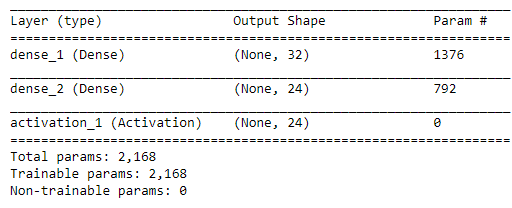
\includegraphics[width=0.9\textwidth]{images/modelo/summaryModel.PNG}
\caption{Resumen del modelo.}
\label{figure15}
\end{figure}

\begin{figure}[h]
\centering 
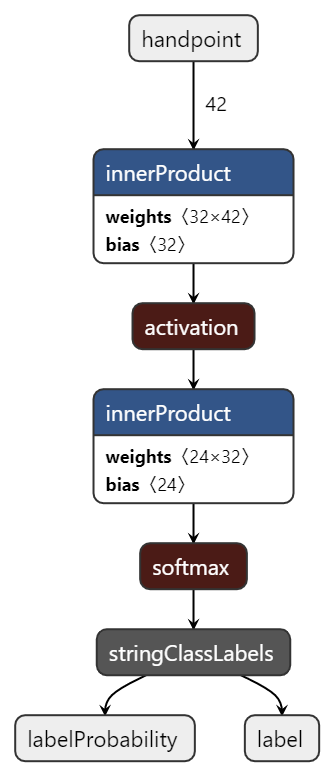
\includegraphics[width=0.3\textwidth]{images/modelo/ASLHandPointTFG.png}
\caption{Capas del modelo.}
\label{figure16}
\end{figure}

\subsection{Entrenamiento}

Se procede al entrenamiento del modelo hasta que se produzcan varias iteraciones consecutivas en el que su porcentaje de acierto en el dataset de validación no mejora. Cuando esto ocurra, procedemos a bajar el hiper parámetro Learning Rate a la mitad y volvemos a realizar el entrenamiento.

\begin{lstlisting}[style=stylepython]
histories.append(model.fit(
    X_train, 
    Y_train, 
    batch_size=batch_size, 
    epochs=200, 
    validation_data=(X_val, Y_val),
    callbacks=my_callbacks,
    class_weight=class_weight_dic))
    
#finetuning
K.set_value(model.optimizer.lr,
                K.get_value(model.optimizer.lr) / 2)
\end{lstlisting}

Este proceso varía de una ejecución a otra porque los pesos iniciales del modelo son elegidos arbitrariamente, en este ejemplo se consiguió un porcentaje de acierto en el dataset de validación de 94.754\% \ref{figure17}

\begin{figure}[h]
\centering 
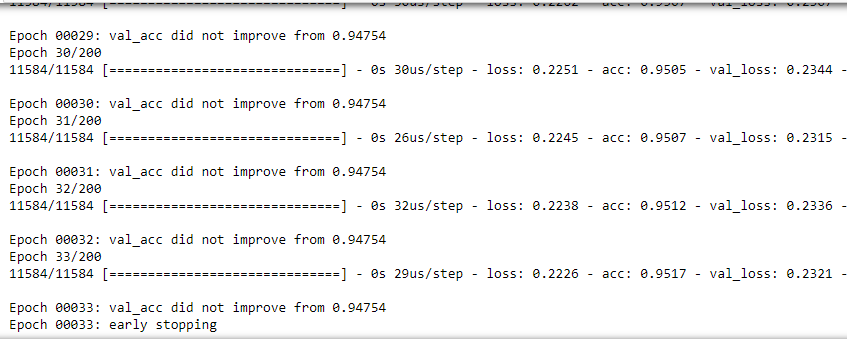
\includegraphics[width=1\textwidth]{images/modelo/validation.PNG}
\caption{Resultados del entrenamiento del modelo.}
\label{figure17}
\end{figure}

\newpage

\subsection{Convertir a CoreML}

Como último paso, tendremos que convertir el modelo a un formato compatible con iOS: Esto se realiza con CoreMLTools \cite{COREMLTOOLS}
Cargamos el modelo con el mejor resultado del entrenamiento, y mediante esta herramienta lo convertimos a CoreML \cite{COREML}.

El modelo tendrá una entrada llamada 'handpoint' que será un vector de 42 valores, y tendrá dos salidas:
\begin{itemize}
    \item labelProbability: Distribución de probabilidad de 24 valores, en el que cada valor representa la probabilidad de que la entrada represente esa letra.
    \item label: Letra con la mayor probabilidad de acierto.
\end{itemize}
 \newpage
 
\begin{lstlisting}[style=stylepython]
import coremltools
from keras.models import load_model
best_model = load_model(checkpoint_dir + "featuresTFGNotebook-0.2425-0.9475.hdf5")
coreml_model = coremltools.converters.keras.convert(
        best_model,
        input_names="handpoint",
        output_names="labelProbability",
        predicted_feature_name="label",
        class_labels=labels)

# add metadata to the model
coreml_model.author = "Daniel Gallego Peralta"
coreml_model.license = "Public"
coreml_model.short_description = "Hand points classifier for 24 different letters of ASL"

coreml_model.input_description["handpoint"] = "normalized coordinates for hand points"
coreml_model.output_description["labelProbability"]= "Prediction probabilities"
coreml_model.output_description["label"]= "Class label of top prediction"

coreml_model.save("ASLHandPointTFG.mlmodel")
\end{lstlisting}

Este archivo 'ASLHandPointTFG.mlmodel' se genera en el directorio actual del notebook y es el modelo en formato CoreML de Deep Learning que utiliza la aplicación iOS.

\end{document}
